\begin{activity} \label{A:11.7.3} 

\ba
	\item Set up and evaluate the triple integral of $f(x,y,z) = x-y+2z$ over the box $B = [-2,3] \times [1,4] \times [0,2]$.

	\item Let $S$ be the solid cone bounded by $z = \sqrt{x^2+y^2}$ and $z=3$. A picture of $S$ is shown at right in Figure \ref{F:11.7.Cone_and_Cone_proj}. Our goal in what follows is to set up an iterated integral of the form
\begin{equation} \label{eq:11.7.TI_not_box}
\int_{x=?}^{x=?} \int_{y=?}^{y=?} \int_{z=?}^{z=?} \delta(x,y,z) \, dz \, dy \, dx
\end{equation}
to represent the mass of $S$ in the setting where $\delta(x,y,z)$ tells us the density of $S$ at the point $(x,y,z)$. Our particular task is to find the limits on each of the three integrals.
\begin{figure}[ht]
\begin{center}
%\resizebox{!}{2.4in}{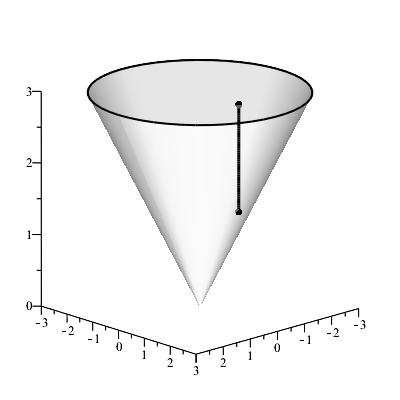
\includegraphics[trim=0cm 1cm 0cm 1.5cm, clip]{11_7_Cone_ex}}
    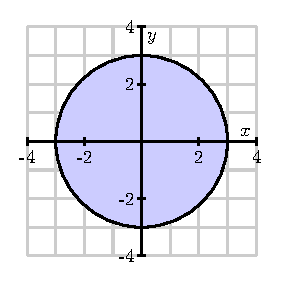
\includegraphics{figures/fig_11_7_cone_project.eps}
  \hspace{1.0in}
%\resizebox{!}{2.4in}{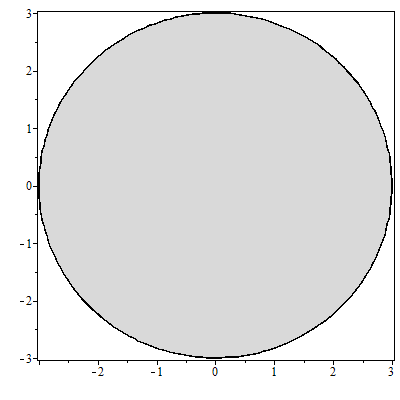
\includegraphics{11_7_Cone_proj}}
  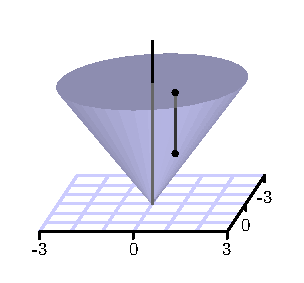
\includegraphics{figures/fig_11_7_cone.eps}
\caption{At right, the cone; at left, its projection.}
\label{F:11.7.Cone_and_Cone_proj}
\end{center}
\end{figure}
%crop graphics in animate trim=<left> <bottom> <right> <top>, clip with includegraphics

	\begin{enumerate}[i.]
	\item If we think about slicing up the solid, we can consider slicing the domain of the solid's projection onto the $xy$-plane (just as we would slice a two-dimensional region in $\R^2$), and then slice in the $z$-direction as well. The projection of the solid is onto the $xy$-plane is shown at left in Figure \ref{F:11.7.Cone_and_Cone_proj}. If we decide to first slice the domain of the solid's projection perpendicular to the $x$-axis, over what range of constant $x$-values would we have to slice?  

    \item If we continue with slicing the domain, what are the limits on $y$ on a typical slice?  How do these depend on $x$?   What, therefore, are the limits on the middle integral? 
    
    \item Finally, now that we have thought about slicing up the two-dimensional domain that is the projection of the cone, what are the limits on $z$ in the innermost integral? Note that over any point $(x,y)$ in the plane, a vertical slice in the $z$ direction will involve a range of values from the cone itself to its flat top.  In particular, observe that at least one of these limits is not constant but depends on $x$ and $y$.

    \item In conclusion, write an iterated integral of the form (\ref{eq:11.7.TI_not_box}) that represents the mass of the cone $S$.

	\end{enumerate}

    \ea

\end{activity}

\begin{smallhint}

\end{smallhint}
\begin{bighint}

\end{bighint}
\begin{activitySolution}
\ba
    
\item
As an iterated integral we have
\begin{align*}
\int \int \int_B f(x,y,z) \, dV &= \int_{-2}^3 \int_1^4 \int_0^2 x-y+2z \, dz \, dy \, dx \\
	&= \int_{-2}^3 \int_1^4 \left. \left[ (x-y)z+z^2\right] \right|_0^2 \, dy \, dx \\
	&= \int_{-2}^3 \int_1^4 2(x-y)+4 \, dy \, dx \\
	&= \int_{-2}^3 \left. \left[2xy-y^2+4y\right] \right|_1^4 \, dx \\
	&= \int_{-2}^3 6x-3 \, dx \\
	&= \left. \left[3x^2-3x\right] \right|_{-2}^3 \\
	&= 0.
\end{align*}

    
\item 
	\begin{enumerate}[i.]
	\item The values of $x$ run from $-3$ to $3$.

    \item The projection of the cone $S$ onto the $xy$-plane is image of the top of the cone, or the equation $\sqrt{x^2+y^2} = 3$. This is the circle $x^2+y^2 = 9$. The limits on $y$ are from the bottom of the circle to the top, or $-\sqrt{9-x^2} \leq y \leq \sqrt{9-x^2}$. 

	\item Notice that the smallest value of $z$ on each slice is on the cone, and the largest value of $z$ is on the plane $z=3$. So the limits on $z$ are $\sqrt{x^2+y^2} \leq z \leq 3$.
	
    \item An iterated integral that represents the mass of the cone $S$ is
\[  \int_{-3}^3 \int_{-\sqrt{9-x^2}}^{\sqrt{9-x^2}} \int_{\sqrt{x^2+y^2}}^{3} \delta(x,y,z) \, dz \, dy \, dx.\]
	\end{enumerate}
    \ea
\end{activitySolution}

\aftera
